\documentclass[11pt]{article}
\usepackage[margin= 1in]{geometry}
\usepackage{cite,times,amsmath,algorithm,algorithmic,cases}
\usepackage{graphicx}
\usepackage{grffile}
\usepackage{indentfirst}
\usepackage{tabularx}
\begin{document}
\title{Analysis of Climatological Data}
\author{ Hesham Salman\\Central Michigan University\\salma1hh@cmich.com
\and Xiaoying Yu\\Central Michigan University\\yu3x@cmich.edu
\and Ting Li\\Central Michigan University\\li2t@cmich.edu
\and Gongzhu Hu\\Central Michigan University\\hu1g@cmich.edu
}
\maketitle
\newpage

% TODO:
%
% Read The Paper Sections And Summarize
%
\begin{abstract}
Each day thousands of locations track and climatological data. This data, when viewed in large numbers can be used to uncover patterns and associations between climatological phenomenon. We hypothesized that elevation had some bearing on the departure from the normal monthly temperature and precipitation. We created a classifier for the general weather patterns of the United States in 2014, and were able to cluster the information to find groups.
\end{abstract}
\newpage

\section{Introduction}
Climatological data is well among the most well catalogued data sources. Most communities catalogue their weather, and many have for centuries! Among the many attributes that have been recorded are temperature, barometric pressures, humidity, and precipitation. This data can be used to uncover local and long-term patterns in weather trends.

Among the many available sources of data is the National Oceanic and Atmospheric Administration (NOAA)\cite{center2010national}. NOAA collects and stores data from multiple sources, including: daily weather forecasts, severe storm warnings, and climate monitoring agencie \cite{center2010national}. The subset of data that we pulled included the following data metrics: Station Name, Departure from Normal Monthly Temperature (DPNT), Departure from Normal Monthly Precipitation (DPNP), Latitude, Longitude, Elevation, and many others. This data set includes data from over 5,000 stations in the United States, with monthly data from January-November of 2014.

We pruned the data set to focus on a number of attributes. The primary attributes that we considered in our data set were latitude, longitude, elevation, DPNP, and DPNT. These values went through a series of data cleaning and verification using Java. After cleaning, the test data set was 61,784 tuples in size. This data set was split into testing and training sets, and, using Python, was converted from CSV format to Aircraft Rescue and FireFighting (ARFF) format for processing in Weka\cite{hall2009weka}. Weka is the primary tool that we used to mine for association rules, classify and cluster the data. Other tools used include Data-Driven Documents (D3js) for data visualizations, Atom Text Editor, and Microsoft Excel for data processing.

We hypothesized that elevation would have some impact on the departure from the normal temperature. Based on this hypothesis, several steps were taken to confirm or deny it. The data points were clustered and classified.


\section{Data Cleaning and Normalization}
The data obtained from NOAA had nine attributes, and over 62,000 total tuples. The data required some pre-processing, as there were 262 unknown values in the station, longitude or latitude value sets. These tuples were removed from the data set. Furthermore, there were 12,759 records containing a -9999 value in the DPNT or DPNP fields. -9999 is the equivalent of an unknown value for this data set. These values were replaced with a zero-value because zero implies no change from the historical monthly precipitation or temperature.


\subsection{Data Cleaning}
When missing geographic data was encountered (latitude, longitude, elevation), the data entry with the missing value was removed from the data set; the Complete-Case method was utilized\cite{han2006data}. The data tuples were removed using ad-hoc methods: the -9999 values were replaced with 0. An unintended side effect of this method is that it skews data towards the center.


\subsection{Data Normalization}
In order to compare the data on equal terms, the data had to be normalized. Only the primary attributes were normalized. All of the primary attributes were normalized through calculation of Z-Score:
\eqref{z-score}.
\begin{equation}
Z-score = \frac{v-\mu}{\delta} \label{z-score}
\end{equation}
where $\mu$ and $\delta$ are thet mean and standard deviation of attribute $v$.

Each attribute was calculated in the following manner. The average of each primary value was calculated as $\mu$. Second, the absolute distance from the average value ($|v-\mu|$) to calculate the absolute values of each attribute. Then, the average mean distance is calculated, in accordance to the absolute mean distance formula:
\eqref{absolute_mean}
\begin{equation}
Absolute Mean Deviation = \frac{\sum{|x - \mu|}}{N}
\label{absolute_mean}
\end{equation}

Specifically, each attribute was calculated in the following steps. First of all, the average of DPNT / DPNP / elevation / longitude / latitude are calculated as $\mu$. Secondly, we apply $|v-\mu|$ to calculate the absolute values of each attribute. Then, we get the average of these absolute values, which is taken as standard derivation $\delta$. Finally, we apply Equation\eqref{z-score} to calculate the Z-score.

\section{Association}

To prepare the data for association mining, we split the data set into 11 distinct sets, each one a separate month. This was done so that patterns on a small scale could be easily identified.

In Weka, we set our support level to 0.1 and the confidence value to 0.6. For each month, we pick up the association rules that include information about DPNP (departure from normal precipitation) or DPNT (departure from normal temperature) implied by Elevation.  Association rules found in January are given as an example in the following:

\begin{enumerate}
\item DPNT Class= Very Cold 658 ==$>$  Elevation Class= Normal 633    conf:(0.96)
\item DPNT Class= Cold  DPNP Class= Normal 705 ==$>$  Elevation Class= Normal 622    conf:(0.88)
\item DPNT Class= Normal  Elevation Class= Normal 1624 ==$>$  DPNP Class= Normal 1392    conf:(0.86)
\item DPNT Class= Cold 1047 ==$>$  Elevation Class= Normal 846    conf:(0.81)
\item DPNT Class= Normal 2714 ==$>$  DPNP Class= Normal 2178    conf:(0.8)
\item Elevation Class= Normal 3545 ==$>$  DPNP Class= Normal 2763    conf:(0.78)
\item DPNT Class= Cold  Elevation Class= Normal 846 ==$>$  DPNP Class= Normal 622    conf:(0.74)
\item DPNT Class= Cold 1047 ==$>$  DPNP Class= Normal 705    conf:(0.67)
\item DPNP Class= Normal 4137 ==$>$  Elevation Class= Normal 2763    conf:(0.67)
\item DPNT Class= Normal  DPNP Class= Normal 2178 ==$>$  Elevation Class= Normal 1392    conf:(0.64)
\item Elevation Class= Low 965 ==$>$  DPNT Class= Normal 591    conf:(0.61)
\end{enumerate}

Using the association rules above, we visualized the frequency of these rules using a Gantt chart visualization, generated in D3. The Gantt chart visualization shows the date on the X axis, wherein each interval represents a month. The Y-axis tracks the elevation of the recording.

%

According to the Association Rules that we gather from Weka, the relationship between Elevation and DPNP is summarized in Gantt Chart and the specific view is showed in Figure \ref{fig:Gantt Chart for DPNP}. Empty spaces in the chart indicate months in which the rules were not observed.

\begin{figure}
  \centering
  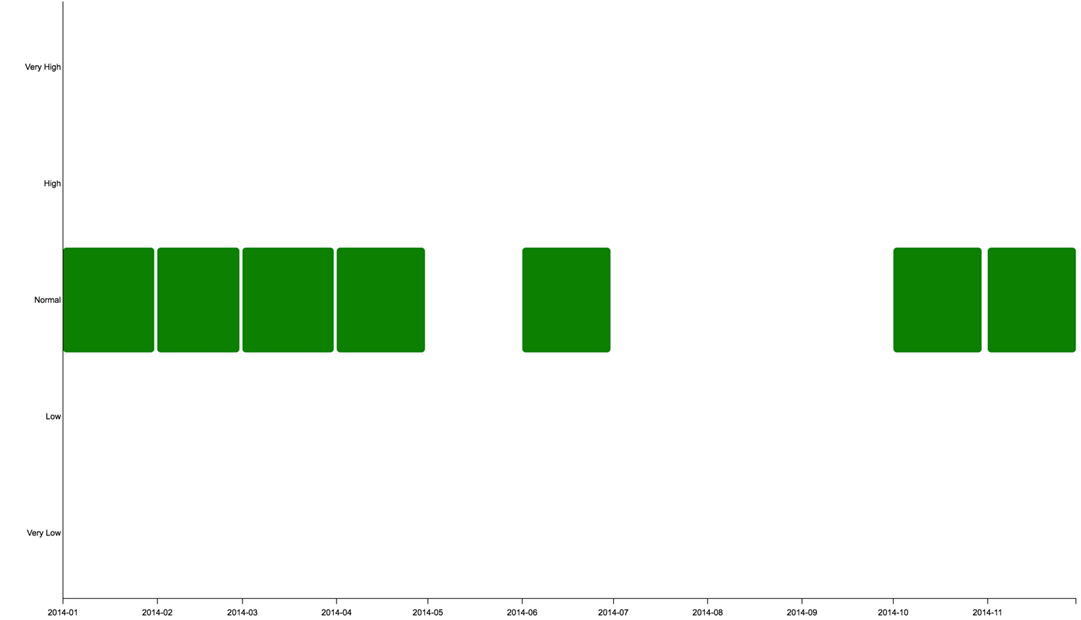
\includegraphics[width=\textwidth]{fig/ganttchart-dpnp.png}
  \caption{In Elevation-DPNP Cantt Chart DPNP Rule Chart, Green=Normal}
  \label{fig:Gantt Chart for DPNP}
  \vspace{-0.1 in}
\end{figure}

\begin{table}
\centering
\begin{tabularx}{\textwidth}{|X|X|X|}
  \hline
  \textbf{DPNP} & \textbf{DPNT} & \textbf{COLOR}\\
  \hline\hline
  Very Wet & Very Hot & Red\\
  \hline
  Wet & Hot & Yellow\\
  \hline
  Normal & Normal & Green\\
  \hline
  Dry & Cold & Blue \\
  \hline
  Very Dry & Very Cold & Black \\
  \hline

\end{tabularx}
\caption{DPNP,DPNT class values and their related color in Gantt Chart}
                \label{table:DPNP-DPNT-COLOR}
                \end{table}
%

As we can see from the Elevation-DPNP visualization, in most of the months, such as January, February and March, when the Elevation value is Normal, the DPNP value tends to be Normal too. Information in this visualization infers that for the locations which have a Normal elevation, their departure from normal precipitation and temperature tend to be Normal too.

We also showed the relationship between Elevation and DPNT in Gantt Chart, and the final result is presented in Figure \ref{fig:Gantt Chart for DPNT}.

\begin{figure}
  \centering
  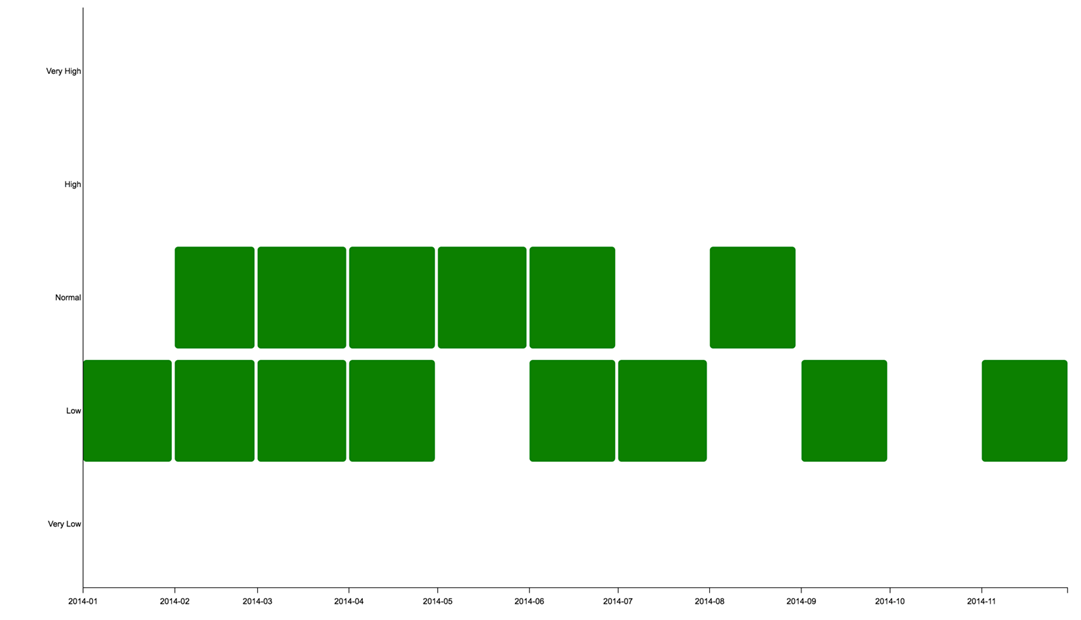
\includegraphics[width=\textwidth]{fig/ganttchart-dpnt.png}
  \caption{In Elevation-DPNT Cantt Chart,while location's Elevation is Low or Normal, its DPNT class value tends to be Normal}
  \label{fig:Gantt Chart for DPNT}
  \vspace{-0.1 in}
\end{figure}

\section{Classification}

The mined association rules are focused on three attributes: elevation, DPNP, and DPNT. In order to find interesting patterns and occurrences in our data-set, we took advantage of the Weka classifier. The classifier we used was a simple Bayesian classifier, and we focused it on five attributes: elevation, latitude, longitude, DPNP, and DPNT. In order to use the classifier, we used the split testing and training sets generated earlier. When setting up the J48 Tree algorithm, we set the confidence level to 0.6 and received the following results:

\subsection{DPNP}
There are 152 classifiers about DPNP in total, and among which, 44 indicates that some locations\rq DPNP class values are Very Wet or Very Dry, others locations are all keep normal.  In the 44 interesting classifiers, we find that in Partial South of America which have a low Elevation, while their DPNT class values are Very Warm, their DPNP class values tend to be Very Dry. The detailed classifiers information is showed as follows:

Elevation Class = Low---Latitude Class = Far South---DPNT Class = Very Warm---Longitude Class = Central:  Very Dry

Elevation Class = Low---Latitude Class = Far South---DPNT Class = Very Warm---Longitude Class = West:  Very Dry

Elevation Class = Low---Latitude Class = Far South---DPNT Class = Very Warm---Longitude Class = East:  Very Dry

Elevation Class = Low---Latitude Class = Far South---DPNT Class = Very Warm---Longitude Class = Far East:  Very Dry.

Hence, we can learn from these classifiers that places in Partial South of America, which have a Low elevation, they are becoming warmer and drier comparing to the previous 20 years’ normal temperature and precipitation.

Meanwhile, some other classifiers tell us that some places are becoming wetter, such as the following ones:

Elevation Class = Normal---Longitude Class = Far East--- DPNT Class = Warm--- Latitude Class = South:  Very Wet

Elevation Class = Normal---Longitude Class = Far East--- DPNT Class = Warm--- Latitude Class = North:  Very Wet

Elevation Class = Normal---Longitude Class = Far East--- DPNT Class = Warm--- Latitude Class = Far North:  Very Wet

As we can see that these places belong to South East or North East America, while their elevation class values are all Normal, their DPNT class values will be Warm.

\subsection{DPNT}

There are 126 classifiers in total, among these 126 classifiers, we find that 93 classifiers imply DPNT value is normal, and there are also some interesting classifiers we find from the result. Such as in North West or Central West of American, while the DPNP class is Very Dry, no matter the Elevation class is Low, Normal, High or Very high, their DPNT class values are all warm or very warm, which indicates that these place are becoming warmer and drier comparing to previous 20 years’ normal temperature and precipitation, the detailed classifiers are showed as following:

Longitude Class = West--- DPNP Class = Very Dry--- Latitude Class = North--- Elevation Class = Low:  Very Warm

Longitude Class = West--- DPNP Class = Very Dry--- Latitude Class = North--- Elevation Class = Very High:  Very Warm

Longitude Class = West--- DPNP Class = Very Dry--- Latitude Class = North--- Elevation Class = Normal:  Very Warm

Longitude Class = West--- DPNP Class = Very Dry--- Latitude Class = North--- Elevation Class = High:  Warm

Longitude Class = West--- DPNP Class = Very Dry--- Latitude Class = Central--- Elevation Class = Very High:  Warm

Longitude Class = West--- DPNP Class = Very Dry--- Latitude Class = Central--- Elevation Class = Normal:  Very Warm

Longitude Class = West--- DPNP Class = Very Dry--- Latitude Class = Central--- Elevation Class = High:  Very Warm




\section{Clustering}
Clustering the data allowed insights into the distribution of the data points and the identification of different groups. The groups were clustered on two parameters: DPNT, and DPNP. Before clustering, the data set was divided into a training set and a testing set. In order to split the data, the data sets were processed by a Java program which had a 68.3\% chance of selecting each data point for the training set (with replacement). Values had a 32.7\% chance of being selected for the testing set. Only normalized data points were used for the clustering of values. Clustering was carried out with the Simple K Means algorithm, with the intention of finding five clusters for DPNT and DPNP. The reasoning behind five clusters is so that areas can be described as being average, above/below average, far above/below average in temperature and precipitation.

The five cluster centroids are as follows:
\begin{itemize}
\item Cluster 0: Very Warm. Cluster Centroid: 2.3173
\item Cluster 1: Very Cold. Cluster Centroid: -2.3277
\item Cluster 2: Warm. Cluster Centroid: 0.8876
\item Cluster 3: Average. Cluster Centoid: -0.0699
\item Cluster 4: Cold. Cluster Centroid: -1.0415
\end{itemize}
DPNP was classified very similarly, with five classifications: Very Dry, Dry, Average, Wet, and Very Wet. The five cluster centroids are as follows:
\begin{itemize}
\item Çluster 0: Dry. Cluster Centroid -1.6818
\item Cluster 1: Very Dry. Cluster Centroid: -10.168
\item Cluster 2: Very Wet. Cluster Centroid: 19.092
\item Cluster 3: Wet. Cluster Centroid: 4.4046
\item Cluster 4: Average. Cluster Centroid: 0.2841
\end{itemize}
\begin{figure}
\centering
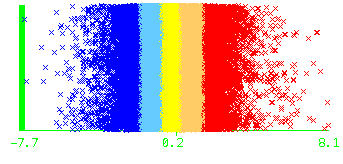
\includegraphics[width=10cm]{dpnt_cluster}
\caption{Clustering of DPNT. From Left to right, the clusters are: Very Cold, Cold, Average, Warm, Very Warm}
\label{fig:dpnt_cluster}
\end{figure}

\begin{figure}
\centering
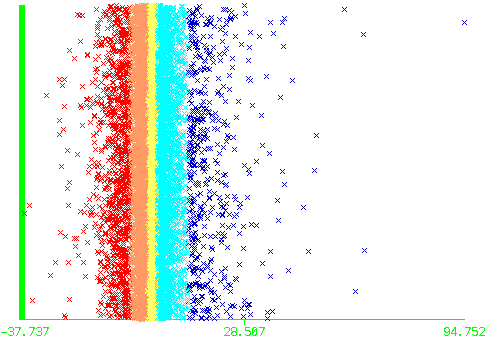
\includegraphics[width=10cm]{dpnp_cluster}
\caption{Clustering of DPNP. From Left to right, the clusters are: Very Dry, Dry, Average, Wet, Very Wet}
\label{fig:dpnp_cluster}
\end{figure}


The distribution in figure \ref{fig:dpnt_cluster} is such that very warm cluster contains ~10\% of the data (6195 data points), the warm cluster accounts for ~29\% of the data (17756 data points), the average cluster accounts for ~28\% of the data(17235 data points), the cold cluster accounts for ~24\% of the data (14729 data points) and the very cold cluster accounts for ~9\% of the data (5869 data points). The distribution in figure \ref{fig:dpnp_cluster} is such that very dry cluster contains ~2\% of the data (1157 data points), the dry cluster accounts for ~27\% of the data (16785 data points), the average cluster accounts for ~63\% of the data(38992 data points), the wet cluster accounts for ~7\% of the data (4336 data points) and the very wet cluster accounts for ~1\% of the data (1157 data points).

In general, 2014 tended to be dryer and warmer than previous years. Variations within each group also existed. Areas with less precipitation tended to be warmer, and areas that had more precipitation tended to be colder, as can be seen in figure \ref{fig:class_distributions}. The differences between each of these classes are significant, having passed a chi-square test with a p-value of 0.01.

\begin{figure}
\centering
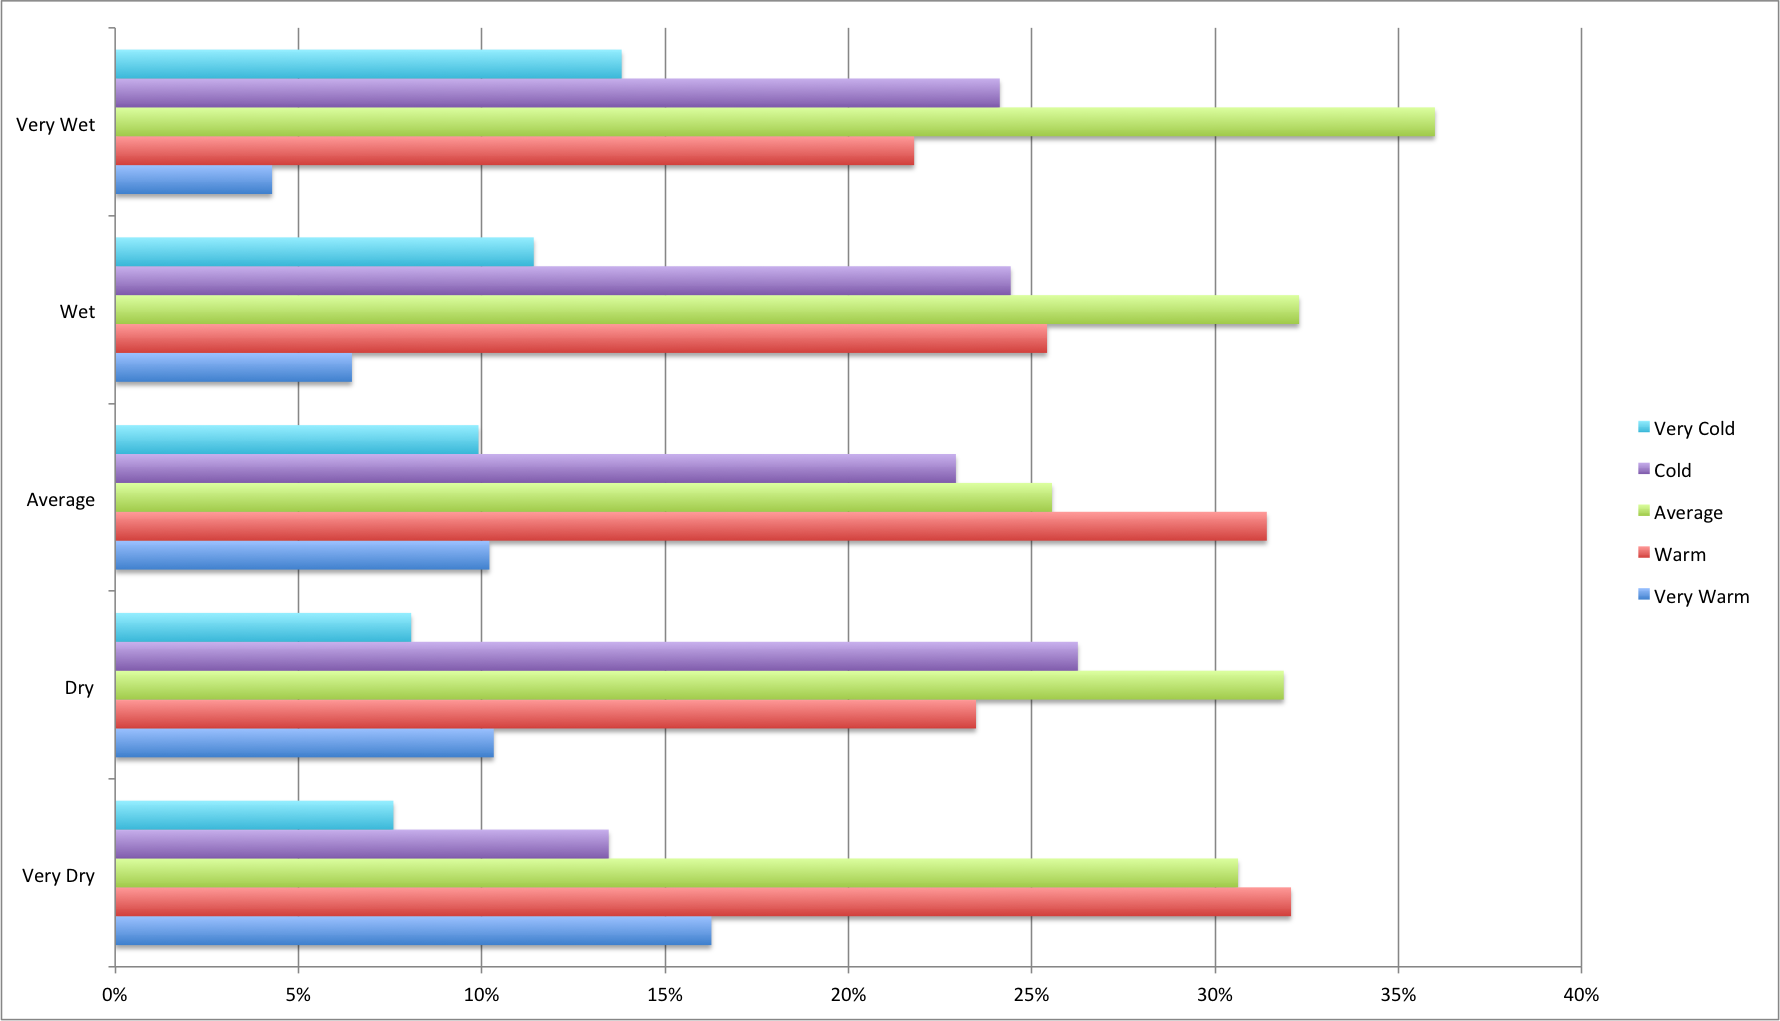
\includegraphics[width=10cm]{ClassDistributions}
\caption{The distributions of temperature within each precipitation cluster}
\label{fig:class_distributions}
\end{figure}


\section{Conclusion}

In our clustering, we were able to conclude that the DPNT and DPNP are somewhat correlated, wherein a warmer locale will tend to be dryer and a colder locale will tend to be wetter. The clustering was unable to conclusively find a correlation between elevation and DPNT or DPNP. The association found that higher elevation tended to have "normal" values, but that could be caused by a number of confounding variables: there may be missing values replaced with 0s, or the overall number of high-elevation areas is small and may not have a wide enough distribution to observe irregularities.
Through classification, we were able to generalize the year of weather patterns for each area. For example, the north west United States was warmer and drier compared to the previous 20 years of temperature records.

\section{Future Work}
Future analysis could be conducted on drought identification. DPNP could be used to identify areas experiencing a drought, and can be cross referenced with an area's Palmer Drought Severity Index. The classifier could be improved to provide a more accurate model for the data.
\bibliographystyle{plain}
\bibliography{bb}
\end{document}
